%!TEX root = ../thesis.tex

\chapter{Discussion: meaning-making in the Bipolar Forum} \label{chap:discuss-bp}
%\chapter{Discussion and critical reflection} \label{chap:discuss-bp}

In the previous three chapters, the findings of the case study were presented. Following a brief qualitative analysis in Chapter \ref{chap:introdata}, findings were organised according to lexicogrammatical system. \sctext{Mood} and \sctext{Modality} were investigated in Chapter \ref{chap:interpersonal}, showing how \Gls{Forum} \glspl{member} use language as a resource for role\hyp{}relationship formation and maintenance, and for the giving and receiving of information and support. This was followed by an analysis of \sctext{Transitivity} choices, which highlighted longitudinal change in how \gls{Forum} users construe the healthcare journey, both in terms of its processes (\emph{diagnosing}, \emph{being\slash having bipolar}) and participants (including Health Professionals, Friends\slash Family, Other Members and The Self).

In this chapter, I discuss key findings with reference to online health discourse literature reviewed in Chapter \ref{chap:onlinehealth}, and with respect to key concepts in \gls{SFL}, as outlined in Section \ref{sect:sfl}. This chapter therefore focusses on directly addressing Research Questions 1 and 2, which concern \glslink{lexicogrammar}{lexicogrammatical}, \gls{discourse-semantic} and registerial change over the course of membership in the \gls{Forum}. Because discussion was presented alongside findings throughout the previous three chapters, the discussion takes the form of semantically organised summaries. Following this discussion, I provide a critical reflection on the findings of the case study, the theories that inform them, and the tools and methods that generated them.
%todo: rq fixup
%A separate discussion and reflection on tools and methods, designed to answer Research Question 4, is presented in Chapter \ref{chap:discuss-method}.

\section{Addressing Question 1: Lexicogrammatical features at risk}

Answering the first question involves simply summarising what was presented in the previous three chapters. New information is not being presented here. The summary is necessary, however, because the second research question is predicated on the first: \glslink{lexicogrammar}{lexicogrammatical} change must be identified in order to discuss \glspl{discourse-semantic} and register in the \gls{Forum}. 

\subsection{MOOD and MODALITY}

Chapter \ref{chap:interpersonal} detailed \sctext{Mood} and \sctext{Modality} choices over the course of membership in the \gls{Forum}. Imperatives and modalised declaratives rise in relative frequency, while unmodalised declaratives decline. Interrogatives, both modalised and unmodalised, undergo no clear trajectory shift.

The investigation of pronominal Subjects showed a clear shift from first toward second person. Modality was also shown to figure prominently in the \gls{Forum}. Absent consideration of other \sctext{Mood} features, the proportion of clauses modalised by any of four types (\emph{can\slash could}, \emph{will\slash would}, \emph{shall\slash should} and \emph{may\slash might}) increases. In terms of combinations of pronominal Subject and modal Finite, clauses with \emph{you} as Subject, combined with any modal, rise steadily. The major exception is \emph{I would}, which is more common in later stages of membership. The \sctext{Tense} system undergoes less shift, but there is nonetheless an observable trend from a focus on the past toward a focus on the present. \sctext{Polarity} does not show readily interpretable trends in either direction.

\subsection{TRANSITIVITY}

Chapter \ref{chap:experiential} detailed shifting patterns within \sctext{Transitivity} choices. Key participants in early \glslink{post}{contributions} are often emotionally charged (\emph{kill}, \emph{crazy}, \emph{scared}). \emph{Anyone} figures prominently, as a general addressee. In later contributions, jargon terms for health professionals and for medications become very key (\emph{pdoc}, \emph{meds}, \emph{tdoc}). References to the community itself also rise in relative frequency over the course of membership. Shifts in the frequency of lexis denoting The Self, Other Members, Health Professionals and Friends\slash Family were also found. These participant types are also represented as Agents to differing extents longitudinally.

In terms of key processes, \emph{diagnosing} and \emph{thanking} are important within early \glslink{post}{contributions}, while \emph{welcoming}, \emph{hugging} and \emph{loving}, among many others, become more common. The \emph{diagnose} process was investigated in greater detail, and changes in its typical attendant participants and processes uncovered: the healthcare professional figures more prominently in the configuration in later contributions; temporal circumstances become displaced by circumstances of veracity (\emph{recently diagnosed} $\rightarrow$ \emph{correctly diagnosed}). Looking at the configuration of \emph{person $+$ relational process $+$ bipolar}, a shift from \emph{being} to \emph{having} was uncovered. 

\section{Addressing Question 2: Discourse-semantics and register}

With an understanding of which words and wordings undergo change over the course of membership, it becomes possible to discuss what these words and wordings \emph{mean} and \emph{do}---that is, to summarise the semantic and discursive content being realised through the \gls{lexicogrammar}. Most existing linguistic accounts of \glspl{OSG} have centred on analysis of the \gls{discourse-semantic} stratum of language and above. For this reason, it is possible to connect many findings from the case study to key claims made in \gls{OSG} literature. As noted in Chapter \ref{chap:onlinehealth}, however, little \gls{OSG} research has drawn upon the \glslink{SFL}{systemic\hyp{}functional} framework, which differentiates between \glspl{discourse-semantic} as the most abstract part of the content plane, and register as a component of context---that is, the situation type in which the text is produced \cite{halliday_language_1989}. Accordingly, it is necessary at this point to determine the most suitable heading under which to treat key \glspl{theme} uncovered during the analysis. For the purposes of this discussion, therefore, phenomena such as \emph{representation of social actors}, \emph{advice}, \emph{references to (in)stability} or the \emph{construal of diagnosis} are treated as primarily \gls{discourse-semantic}; member roles and identities more generally are registerial.

\subsection{Discourse-semantics in the Forum}

During the previous three chapters, \glslink{lexicogrammar}{lexicogrammatical} findings were generally presented alongside a brief explanation of their \gls{discourse-semantic} significance, with findings organised by \glslink{lexicogrammar}{lexicogrammatical} feature, and separated along metafunction lines. The main limitation of this structure is that the discussion of meanings being made by words and wordings becomes disjointed: meanings are made through different grammatical systems and subsystems that are deployed together in text as it unfolds. In fact, language is structured around meaning, and simply realised through words and wordings \cite{halliday1978language}. The structuring of findings into \sctext{Mood} and \sctext{Transitivity} chapters therefore does not allow sufficient space for a discussion of the meanings made by hierarchical or agnate linguistic structures. Moreover, there are a number of moments where meaning\hyp{}making transcends the systemic division of metafunctions. To coherently discuss meaning\hyp{}making in the \gls{Forum}, therefore, a discussion organised semantically is now required.

\subsubsection{Social actors and interactants in the healthcare journey}

A useful starting point in a summary of \glspl{discourse-semantic} in the \gls{Forum} is to broadly characterise the kinds of social actors and interactants that occur, and the kinds of processes they are construed within, without respect to longitudinal change \cite{van_leeuwen_representation_1996}. By collapsing participant heads into four groups, the \sctext{Transitivity} analysis differentiated between four main categories of social actor: \emph{The Self}, \emph{Other Members}, \emph{Health Professionals} and \emph{Friends\slash Family}. These participant types are construed within different processes: The Self is very commonly a Senser (engaging in \emph{appreciating}, \emph{thinking}, \emph{guessing}, \emph{hoping}, \emph{knowing}), but is rarely construed as the Sayer. Health professionals, on the other hand, do a great deal of saying, telling, and asking---in fact, they are involved in verbal processes more than twice as often as any other participant type. Of course, this distribution of Process Type over participant type aligns with any sensible expectation of how \gls{consumer} health discourse serves to represent the stakeholders in healthcare journeys. Because language mediates most critical events in clinicians' treatment of mental health issues (diagnosis, prescription, therapy and directives, to name just a few examples), health professionals are often construed as Sayers. Friends and relatives are unsurprisingly construed relationally, as their relevance within \glslink{member}{Forum users}' medical narratives is largely determined by their relationship to the speaker. The self is construed more often than other participant types as thinking because people only have direct access to their own cognitive processes; others' thoughts must be inferred from their verbal, behavioural and material actions.

The way these four types of Things are construed undergoes change over the membership course. First, in terms of their overall prominence as experiential participants and interpersonal Subjects, there is a steady decline in the relative frequency of first person, and a steady increase in the relative frequency of second person\slash references to Other Members. Interpersonally, this can be analysed in two ways. First, it can be seen as a shift from \glslink{member}{users} charging themselves with modal responsibility to charging their addressees, over whom they have a kind of authority conferred by their membership stage. In this analysis, \glslink{member}{users} make cases for their own membership within communities \cite{stommel_use_2011,vayreda_social_2009}, and, upon the ratification of their bid, shift toward examining the claims made by later newcomers \cite{paulus_`please_2015}. Such a shift would be more dramatic still if the rise in imperative clauses were taken into account: in imperatives, it is the second person, despite being absent in the \gls{lexicogrammar}, that is held responsible for meeting the speaker's demand. The second, complementary analysis is that the interpersonal burden is always on newcomers---as a \gls{member} exits newcomer membership stages, he\slash she begins to charge newer \glspl{member} with the interactive demands that he\slash she has recently shed. The newcomers, in occupying the Subject role, are always the dominant `resting point of the argument' \cite[p.~118]{halliday_introduction_2004} within \gls{Forum} exchanges. Ideationally, the world being represented through language is, in the same way, the world of the newcomer: as \glspl{member} progress toward veteran roles, their representations of their own health journeys become less frequent, and shift in purpose, serving more often as exempla from which newcomers can learn about common mistakes or useful strategies in the management of \gls{bipolar} \cite{pfeil_social_2011}. To borrow terminology from \textcite{bauman1990poetics}, \glslink{member}{users} shift longitudinally from entextualisation of the Self toward entextualisation of the Other. 

Though The Self and Other \glspl{member} are on divergent trajectories in terms of relative frequency as participants, both are positioned as Agents to very similar extents (69.31\% and 71.19\%, compared with Health Professionals and Friends\slash Family, at 77.68\% and 65.78\% respectively). This shows us that while propositional validity rests predominantly on the newcomer, and while the newcomer's journey is typically the thing being construed by newcomer and veteran alike, both newcomer and veteran, as social actors in healthcare journeys, are represented as causing change to approximately the same degree. The Self and Other \Glspl{member} occupy distinct roles within the interactions of the \gls{Forum}, but more or less the same position within the world of healthcare being represented by \gls{Forum} \glspl{member}. The Self and Other \glspl{member} also undergo very similar increases in the extent to which they are positioned as Agents: in newcomers' talk, both are positioned as media through which processes happen; in veteran talk, increasingly often, The Self and Other \glspl{member} are construed as Things that say, think, act or do. This represents a shifting understanding of the role of the \gls{consumer} within the healthcare journey, from passive experiencer of healthcare systems to navigator of the journey's trajectory. Simply put, the longer a member contributes to the \gls{Forum}, the more likely he\slash she is to construe both themselves and others as `active patients'.

Meanwhile, Health Professionals undergo very different kinds of change. In terms of overall frequency, they rise rapidly in the final two stages of membership, indicating an increasing emphasis on formal healthcare institutions and their role in \glslink{bipolar}{bipolar} management in veteran talk. At the same time, however, Health Professionals are less and less commonly positioned as Agents. Importantly, the disparity in agency between \glslink{member}{Forum members} (i.e. The Self $+$ Other Members) and Health Professionals lessens over time. Such a shift indicates that veterans construe a less hierarchical professional--\gls{consumer} dynamic than newcomers, and an increasing level of \gls{consumer} empowerment generally. Rather than being Mediums through which processes operate (\emph{My doctor diagnosed me with bipolar}), veterans are instead more likely to cast the \gls{consumer} as interpersonally responsible for making the proposition valid, and, simultaneously, as experientially responsible for progression through the healthcare journey (\emph{You should go to your doc and get a diagnosis}). Veteran \glspl{member} therefore tend to advocate a number of current components of the dominant biomedical ideology, such as \emph{the active \gls{consumer}}, \emph{shared decision making}, and \emph{\glspl{consumercentred}}. %While we do not have evidence to suggest that veteran \glspl{member} actually put into practice the kinds of meanings they construe, we can still ...

\subsubsection{Discursive shifts}

%todo
%Four of these changes---the way diagnosis is framed, the way that \gls{bipolar} is attributed, the increasing frequency of advice, and the shift from instability and negative lexis to stablity and positive lexis, are discussed below.

%\paragraph{Diagnosis}
% The shifts in propositional responsibility and construal of social actors are accompanied by

Other kinds of longitudinal changes in semantics can be identified through shifts in how particular grammatical constituents are typically configured within a text. One of the most striking of these is the way in which \glslink{member}{users} construe the process of diagnosis---a more or less mandatory component of the \gls{bipolar} journey within the biomedical ideology of the \gls{Forum}. \emph{Diagnose} as an Event was found to be a very key process in first \glslink{post}{contributions}, leading to more delicate analysis of its behaviour in the \gls{corpus}. This analysis turned up an increasing rate of grammatical metaphor (in the form of nominalisation, as \emph{diagnosis}), and shifts in attendant participants and circumstances. Each of these changes reflects a change in the \glspl{discourse-semantic} of the Event. First, the metaphorical realisation of the diagnosis Event as a participant opens it up to possession, deixis and more precise kinds of classification. At the beginning of membership, diagnosis is an Event that the speaker experiences, often without his\slash her volition, and often without an explicit Actor. The Event is situated in the past, represented as catalysing the new \glslink{member}{user}'s decision to sign up or contribute to the \glslink{Forum}{board}. Diagnosis, as others have remarked, can function as a kind of entry ticket, or marker of legitimacy, for membership in mainstream \glspl{OSG} \cite{stommel_use_2011}. Within the overarching ideology of the \gls{Forum}, treatment \cite[including the talk therapy provided by \gls{Forum} interaction itself---see][]{kaufman2016producing} is reserved for those who have an official mandate that warrants it \cite{vayreda_social_2009}. As such, it is no surprise that the \emph{diagnose} process is increasingly construed as a Thing that can be given, possessed and inspected. In the \glslink{Forum}{community}, \gls{bipolar} is understood to be treatable, but not curable---the amount of time between the diagnosis and the present is therefore more or less immaterial when inspecting the validity of the entry condition. Instead, what becomes important is the veracity of the diagnosis: \emph{suspected} and \emph{unofficial} diagnoses must become \emph{proper} and \emph{official} diagnoses, because it is correct diagnosis that steers the newcomer on the optimal path within the \gls{bipolar} journey.

The distinction between \emph{being} and \emph{having} \gls{bipolar}, and the shift toward the latter over the membership course, functions differently to the change in the configuration of diagnosis. Employing the \emph{being} form does not put the validity of a membership claim at risk; instead, new \glspl{member}' transgressions of the \emph{having bipolar} norm provide an opportunity for the ideological values of the \glslink{Forum}{community} to be made explicit \cite{weber_missed_2011}. More specifically, veteran \glspl{member} can use the moment to semiotically reconfigure \emph{bipolar} into something that can be controlled, and thus, can be managed, be it by medication, visits to a health professional, or the talk therapy that constitutes \gls{Forum} interaction itself.

%todo: too long first half of this paragraph
Another area of change is the increasing frequency of advice. Advice is best understood as a \gls{discourse-semantic} phenomenon: it is congruently delivered within individual clauses (or potentially clause complexes), rather than within individual constituents, or across a text more generally. Its deployment may involve explicit lexicogrammatical features (\emph{Let me give you some advice \dots}), but is far more commonly signalled through combinations of \sctext{Mood} and \sctext{Modality} choices, particular Process Types, and so on. It is most easily recognised by its semantics, where the addressee is being told that a particular course of action is desirable in the eyes of the speaker. That said, it does have common \glslink{lexicogrammar}{lexicogrammatical} realisations, in imperatives, modalised declaratives, and, more rarely, interrogatives \cite{locher2006advice}. One point of discussion is whether the membership stage of the veteran member may determine the congruence of chosen realisations of advice \cite{decapua_`if_1995}. On one hand, there is indeed a steady growth in the number of imperatives over the membership course. On the other, hypothetical statements, in the form of modalised declaratives, also become much more common over time. The reason for this is that what develops over the course of membership is not simply an authority over newer \glspl{member} that manifests in more direct realisations of commands---rather, it is a nuanced register designed to best motivate the newcomer to adopt community values that are intended to facilitate better health outcomes. Advice is a coupling of experiential and interpersonal content: suggested action, but also a negotiation of the power dynamic between speaker and addressee (and the wider audience of potential posters and lurkers) \cite{harrison2009politeness}. Given that a clause must have interpersonal and experiential value, this is an expectation within any \glslink{SFL}{systemic-functional} interpretation of text.

%\paragraph{Stability and attitudinal lexis}

%todo: copy edit
A final kind of \gls{discourse-semantic} change is in general preference for construals of stability over instability, and of positive over negative attitudes. These tendencies are the most diffuse of identified semantic change, and fall far closer to the pole of lexis (or instance), than to grammar (or system). This is to be expected: as \textcite{martin_language_2005} explain, the systems of \sctext{Appraisal} are not lexicogrammatical, but semantic, in the first place. For this reason, they did not receive sustained treatment from a lexicogrammatical perspective. Even so, the shifts are striking, occurring as very key participants and processes in the first and last stage of membership. The shift toward construals of \emph{stability} can best be understood with reference to the phenomenology of \gls{bipolar} itself, and with an understanding of the \gls{Forum}'s therapeutic orientation: because \gls{bipolar} involves oscillation between periods of mania and periods of depression, the achievement of stability (of emotions, behaviours, relationships, etc.) is, in a sense, the point at which \gls{bipolar} has been successfully managed. As shown in the previous chapter (Table \ref{conc:stability}), veteran members commonly construe stability as the Goal of a material process, with \gls{Forum} \glspl{member} functioning as the Actor who will eventually \emph{find}, \emph{maintain}, \emph{reach} or \emph{achieve} it. Meanwhile, the gradual elimination of attitudinally negative lexis reflects an increasing tendency to construe the ideal goals of the healthcare journey, rather than previous or potential future problems. This reinforces to newcomers a conceptualisation of \gls{bipolar} as manageable through diligent self\hyp{}regulatory behaviour. The increasing construal of positive action within the community (\emph{hugging}, \emph{welcoming}) builds a representation of the \gls{Forum} as a supportive space in which the journey toward stability can be carried out.

    %The case study did not attempt to uncover, for example, shifts in the ways in which a particular medication, symptom or social actor are appraised, or the kinds of participants likely to figure into processes of \emph{killing}, or the kinds of participants evaluated as \emph{crazy}. Little analysis of attitudinal lexis was performed, not because attitudinal lexis does not make interesting meanings in health context \cite{woodward-kron_international_2016}, but because such patterns are difficult to locate using the methods developed for and applied in the case study.


    %Locher's approach, however, involves manual classification of data for eventual quantification. Manual classification, for \gls{discourse-semantic} phenomena, is more reliable, and sensitive to co-text in a way that automated methods cannot yet be. This sensitivity comes at the cost of automatability and scale.

    %The methods used for the case study cannot match the level of semantic insight that is possible with human annotation. That said, even manual identification of concepts such as \emph{empathy} is not a particularly reliable task, especially when the evidence is based on the analysts impressions ahead of any rigorous \glslink{lexicogrammar}{lexicogrammatical} criteria. For this reason, it seems that further research into advice provision and reception online is (until computational methods for automatic identification of discourse-semantic features) best carried out using a mixed-methods approach, where quantitative accounts of \glslink{lexicogrammar}{lexicogrammatical} features inform texts selected for contextualised analysis, and where results from contextualised analysis can be fed back into automatic querying. Manual classification of advice in a subset of a corpus could be fruitfully used as training data for an automatic text classification approach, as performed by \textcite{maclean_forum77:_2015}.





%todo: use matthiessen's activities map
% The fact that the registerial typology is a continuum is particularly useful---identified longitudinal shifts were typically consistent, and gradual.
%From there, the \emph{register}(s) of the \gls{Forum} can be described,
%and how the transition toward veteran membership may affect the kind of patterns seen within.
%[Register is] the configuration of semantic patterns, that are typically drawn upon under the specified conditions, along with the words and structures that are used in the realization of these meanings \cite[p.~23]{halliday1978language}.
% A register can be defined as the configuration of semantic resources that a member of a culture typically associates with a situation type. It is the meaning potential that is accessible in a given social context \cite[p.~111]{halliday1978language}.
%%that is, to use the understanding of semantics to relate \gls{lexicogrammar} to .
%`relate wording to context via meaning which acts as the interface between the two’ (Hasan 2009a: 182).

%  The first of these two tasks has been comprehensively explored in this thesis.



\subsection{Register}

In the sections above, I have summarised some key parts of a normative semantics that is drawn upon more and more as \glslink{member}{users} progress toward veteran membership. The task that remains is to connect the identified changes in the content plane of interactions within the \gls{Forum} to the contextual variables of field and Tenor.

In \gls{SFL}, \emph{register} is the stratum above, or \emph{realised by}, \glspl{discourse-semantic}. It is, in effect, a type of situation, where the patterns and probabilities of instantiation of particular linguistic features are set \cite{halliday_introduction_2004,lukin2011halliday}.
Following \textcite{matthiessen_applying_2013}, any given healthcare interaction can be understood as existing at the most delicate end of the cline of instantiation---as an instance, or realisation, of the meaning potential of the linguistic system, related to the journey through a common ideational focus on a health\hyp{}related issue, and a common interpersonal interactant, the self. By investigating patterns in a \gls{corpus}, we progress from the (delicate) realisation end to the (broad) system end, locating possibilities and probabilities in the \glslink{lexicogrammar}{grammar}, and relating these to meaning\hyp{}making across the interpersonal, experiential and textual metafunctions. From the sketch of relevant choices along the cline of instantiation, we can then produce a more abstract register description, covering who is talking, what language is being used to construe, and what language itself is doing within the situation. The case study has already presented a quantitative overview of register, in the form of not only shallow features, but in the more delicate syntagmatic behaviour of some of the lexicogrammatical features that differentiate the \gls{Forum} register from others. In the sections below, I add a qualitative description of the Field and Tenor of the \gls{Forum}, with some cautious speculation regarding the unexamined dimension of mode.

%To add it to existing work that has centred on consumers' journeys through hospitals \cite{slade_communicating_2015}, it is necessary to find out how language is used in the Forum, how language use might change over the course of membership, and how this language is similar or different to language in other parts of the journey.

%By relating this to previous and future healthcare interactions, we can build an empirical account of the healthcare journey, and how the various interactions ultimately work together to shape consumers' understanding and decision-making practices.

%meanings within their respective metafunction. From our understanding of \gls{lexicogrammar} and \glspl{discourse-semantic} in the collection of texts, we can formulate a simple register description.

%Matthiessen also highlights the importance of computationally driven registerial mapping, drawing on the work of (e.g.) \textcite{paris_constraining_1991}. For computational linguists, machine readable context models are highly desirable, as semantic phenomena can be more easily predicted when the register of a text is known \cite{paris_constraining_1991}: in an interaction between a health professional and his\slash her client, for example, we can assume that demands made by the client are less likely, when compared with the health professional, to be realised through bare imperatives, as the client's issuing commands in this way may be face\hyp{}threatening.

%\section{Understanding the Bipolar Forum}

%It is useful to begin with a brief description of meaning-potential and meaning-making practices in the Forum. Members' identities are communicated through two main semiotic resources. First, and perhaps primarily, users perform and negotiate identity through linguistic choices made in posts. These posts are presented multimodally within a container of interpersonally meaningful semiotics of a second type: information regarding gender, join date, username and post count, over which the user has little continuing control. The posts themselves, however, have a great deal of longevity: each is immediately archived, and available by reading older threads, or by viewing the user's profile. Their role in the process of interpersonal meaning-making therefore changes over time, shifting from one type of semiotic to another. In the present, a post is directly involved in the unfolding of a thread as an interactive exchange. In the future, though the same text has left the user's control, it becomes a resume of past activity, retaining the potential to inform others' beliefs and behaviour, and thus continuing to figure into the constant negotiation of identity within the board.

%The case study provides a preliminary sketch of an emerging register within a cluster of registers found in the various situations involved in the healthcare journey. It is described below in terms of its Field and Tenor.

\subsubsection{Tenor}

In terms of the Tenor of discourse, the \gls{Forum} is unlike most other possible elements of the consumer journey: unlike formal healthcare settings, where the consumer typically enters into a series of provider--consumer interactions \cite{slade_emergency_2008}, the community presents a space for intra--consumer interaction. In comparison to hospitals, \glspl{member} of the Forum are in a relatively equal role\hyp{}relationship, sharing both an identity (as people living with \gls{bipolar}) and a goal (effective management of symptoms). Equality is in some respects facilitated by the architecture of the website, and text\hyp{}based \gls{CMC} in general, which may obscure a number of demographic distinctions that lead to unequal treatment \cite{walther_computer-mediated_1996}. That said, in line with the work of \textcite{herring_computer-mediated_2001}, the gender, age, and nationality of many \glspl{member} are often easy to disambiguate: many \glslink{member}{users} make their gender visible as a metadata feature that appears to the side of their \glspl{post}; usernames and linguistic choices can also often communicate gender. Moreover, even though role\hyp{}relationships are equal compared to typical provider--consumer interactions, \gls{Forum} \glspl{member} still take on distinct, hierarchical positions within the community. The authority of the veteran over the newcomer, while not absolute, manifests in the lexicogrammatical strategies selected by veterans for advice provision: the modalised declarative \emph{I would} construction is more common than the bare imperative command that may emerge when statuses are very unequal \cite{decapua_`if_1995}. At the same time, the \emph{I would} construction flags the fact that the expertise of the veteran is of a lay, rather than professional type. As noted by \textcite{smithson_membership_2011}, the action content of veteran's advice is typically conservative. Most often, advice serves to reinforce mainstream medical expectations: where newcomers deviate from the biomedical norms, veterans offer advice that bolster the health professional's authority (\emph{I would DEFINITELY recommend seeing a psychologist}; \emph{I would highly recommend that you take your meds on a daily basis.}). Both newcomer and long-term members' interpersonal exchanges can be understood as attempting to negotiate a legitimate position within the social hierarchy of the community \cite{varga2014grieving,koteyko2015performing}. For the newcomer, there is a legitimate need for information and support; for the veteran, it is the existing status at the top of the Forum's social hierarchy that is preserved through interpersonal negotiation.

%This is simultaneously the most useful and most problematic of the legitimacy approach to understanding community dynamics: almost all behaviours can convincingly be argued to be building some kind of legitimacy. 

%It is worth noting that the decision to divide the analysis into Mood and Transitivity parts was made before any exploratory or preliminary engagement with the data. It was therefore a theoretical imposition, based on key hypotheses from systemic grammar (that are indeed not widely shared within mainstream linguistics). The division has indeed proven useful for mapping meaning to wording, and dividing both into distinct metafunctions. That said, because the decision was made prior to analysis, we cannot know for certain whether such a categorisation would have emerged from the data themselves.

% tense?
\subsubsection{Field}

Field is the variable with the most overlap between other components of a consumer's healthcare journey. In the \gls{Forum}, like in a consultation with a doctor, the consumer is likely to talk about symptoms, diagnoses and treatments; related issues such as family, work and hobbies may also be construed. Even within this field, however, for different situations, there will still be differences in the frequencies with which particular participants and processes appear, and the ways they are modified and arranged as configurations and activity sequences. In the Forum, for example, a great deal of talk centres on personal relationships and emotional states. This kind of talk is less likely in some healthcare encounters (e.g. a hospital stay), but more likely in others (e.g. within a psychiatrist's office).

The Field of discourse under discussion by \gls{Forum} \glspl{member} also changes over the course of membership. Users engage in more metadiscourse, opt for jargon variants of common participants, and use vague language to provide advice that can be applied to not just the addressee, but other potential readers. As mentioned earlier, a number of lay and negative Events and Things are gradually displaced with more neutral, scientised language: talk about \emph{mood swings} and \emph{going crazy} declines, while references to \emph{stability} and \emph{balance} rise. Broadly, these changes reflect an increasingly faithful reproduction of the experiential semantics of a biomedical ideology, where the ideal healthcare journey involves a combination of engagement with formal healthcare institutions (for diagnosis, therapy, etc.) and self-monitoring for indicators of potentially oncoming manic\slash depressive cycles. In line with a biomedical model, the \gls{Forum} is framed as a space for a kind of talk therapy that can foster stability by allowing a space where people can vent, reflect, or engage in the exchange of information about Bipolar. It is an important space, but one that ultimately plays a secondary role to what can be accomplished through medication and psychotherapy: only doctors can diagnose or change medication regimens, but veteran \glspl{member} can encourage newcomers to speak with the doctor about their problems. Where newcomers deviate from this normative ideology, as shown by \textcite{weber_missed_2011}, veteran \glspl{member} take the opportunity to make community norms explicit: (\emph{part of the purpose of this space is for venting}; \emph{we aren't docs and can't diagnose you}; \emph{you're not *A* bipolar, we're not things, it's a condition}). The function here is to try to align the newcomer with the normative ideology, and the normative illness trajectory that exists within that ideology.

%todo: needs in text reference
\begin{figure}[htb]
\centering
\addvbuffer[12pt 8pt]{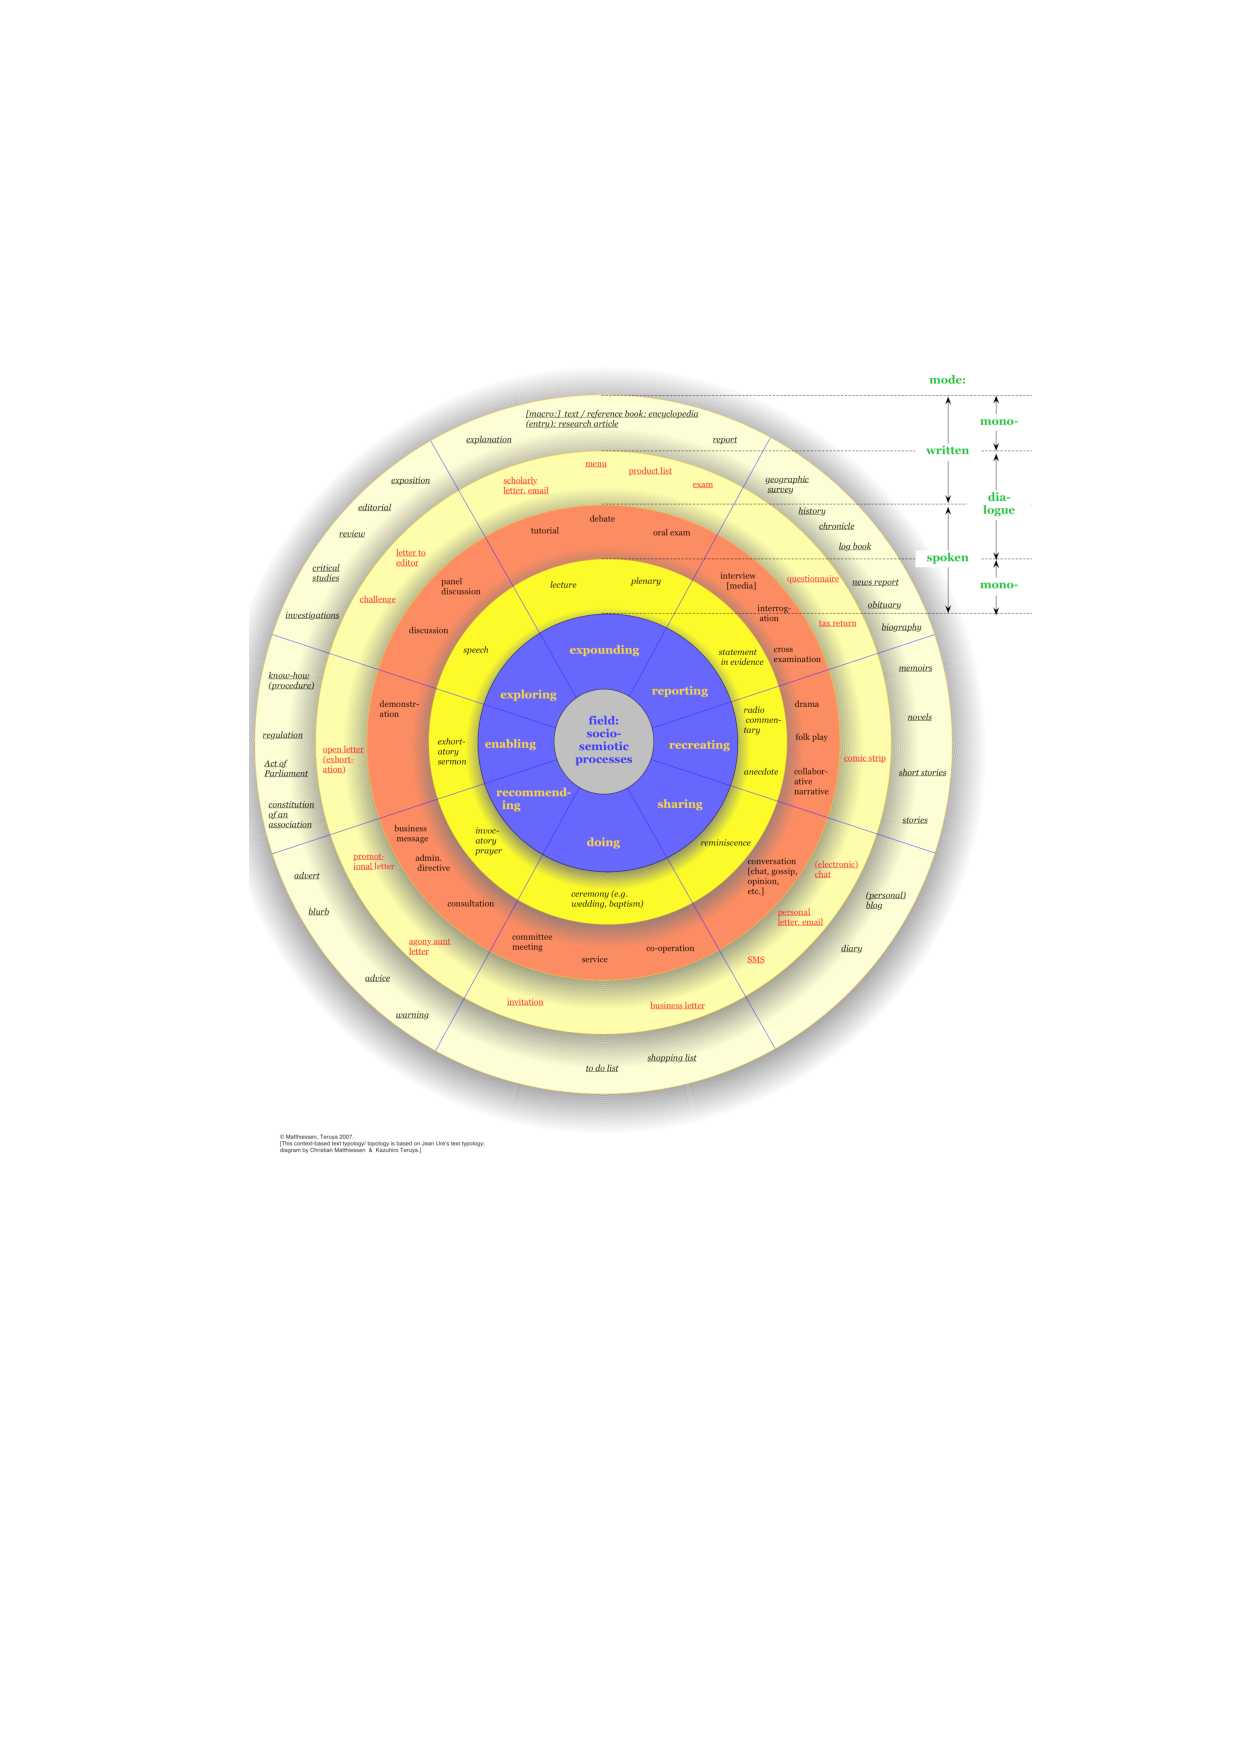
\includegraphics[width=0.66\textwidth]{../images/text-typology.pdf}}
\caption[Socio-semiotic processes]{Socio-semiotic processes as topology (Matthiessen, 2015)}
\label{fig:pie-of-fortune}
\end{figure} 

The overarching changes in field can be represented as shifts in the kinds of socio\hyp{}semiotic processes in which users typically engage (see Figure \ref{fig:pie-of-fortune}). New \glspl{member} engage most commonly in processes of sharing (their medical histories, current concerns and problems, etc.) and in information or support seeking. Though veterans, like newcomers, construe previous experiences from their healthcare journeys, more commonly, they are not simply \emph{sharing}; at the same time, they are \emph{recommending}---they provide, from their own lived experience, examples of previous problems and solutions \cite{koteyko2015performing}. \emph{Recommending} can, of course, also be more direct and explicit, with veteran \glspl{member} routinely issuing demands for material (\emph{find a doctor}), verbal (\emph{communicate with your doctor}) and mental (\emph{consider it a learning experience}) action \cite{pfeil_social_2011}. It is important to remember, however, that a community of the size and scope of the \glslink{Forum}{Bipolar Forum} is bound to become a space for a diverse range of socio\hyp{}semiotic processes. Socio\hyp{}semantic processes of all types were seen during qualitative exploration of the \gls{Forum}: \emph{enabling} can be seen in the sticky \glspl{post} that list community guidelines, \emph{exploring}\slash \emph{expounding} are used to reflect on recent news articles and research about \gls{bipolar}; Some \glslink{member}{users} engage in \emph{recreating} by writing poetry about their inner and outer healthcare journeys. 

%The dimension of \textbf{Mode} differs radically from the kinds of interactions generally studied within \gls{HC}: the Bipolar Forum is computer\hyp{}mediated, written, semi\hyp{}synchronous and many\hyp{}to\hyp{}many, compared with the face\hyp{}to\hyp{}face, spoken, synchronous, one\hyp{}to\hyp{}one interactions analysed by \citeNP{slade_communicating_2015}. A notable affordance of the Mode dimension of the \gls{Forum} is that turn times are unconstrained, with language being used to monologue, diarise, explain or vent. The medium also allows users to reflect and revise before posting, creating cohesive texts, largely free of the kinds of disfluencies that characterise spoken (dialogic) interaction, such as false starts, fillers and repetitions. %Though an analysis of realisations of the \sctext{Mode} dimension was not undertaken due to spatial constraints, methodologically speaking, it is these features are the ones that make \glspl{OSG} a potentially valuable data source for healthcare communication research. The lack of constraints on what can be written mean that large amounts of content are authored on diverse subjects.

%\subsubsection{Mode}

%While the textual metafunction was not investigated, it is still useful to provide a brief discussion of the register dimension of mode. In Chapter \ref{chap:onlinehealth}, I reviewed an argument made by \textcite{crowston_reproduced_2000} that mode of \gls{CMC} can be conceptualised according to their relationship, or lack thereof, with offline modes: some types of \gls{CMC} replicate an offline counterpart, while others reconfigure it. Others still can be classified as `new', having no observable antecedent. If we compare online and offline support groups, it is clear that the register variable undergoing the most change is that of \gls{Mode}: the \gls{Forum}, and \glspl{OSG} in general, are computer\hyp{}mediated, written, semi\hyp{}synchronous and many\hyp{}to\hyp{}many, compared with potential offline counterparts, which are face\hyp{}to\hyp{}face, spoken, synchronous, and limited to smaller groups. Field and Tenor, however, remain for the most part similar.

%Whether or not we can understand the \gls{Forum} as reconfiguring offline support group communication, or as a new register\slash genre entirely, remains difficult to answer. It is likely, for instance, that the vast majority of readers and contributors to the community have never attended a face\hyp{}to\hyp{}face support group, limiting the extent to which they may attempt to reapply patterns from the antecedent to the novel genre. Nonetheless, there is some interaction between online and offline support groups: in earlier stages of membership in the community, attributions of bipolar via \emph{being bipolar} constructions are more common than \emph{having bipolar}. Many of these ascriptions follow the stereotypical self-introduction from Alcoholics Anonymous meetings (and media representations thereof): `Hi, I'm [name], and I'm an alcoholic' \cite{_must_2014}. Moreover, it is worth asking whether it is useful to classify the relationship between online and offline genres in the first place. As noted by \textcite{herring_discourse_2011}, a given genre of \gls{CMC} may not be stable, tending to gravitate toward more novelty as it ages and develops features that cater to the demands of users. This creates a basic contradiction, where what was once seen as reconfigured, after further development, becomes classified as emergent or new, despite having evolved from an offline antecedent genre.







%Medication targets the physiological and biological components of illnesses, while Forum interactions target the social and the semiotic.

%The overarching point here is that \glspl{OSG} exist because they provide needs that are unserved by formal medication infrastructure. \textcite{maclean_forum77:_2015} noted the importance of such spaces for drug abuses aiming for recovery, for whom honest dialogue with health professionals may not be not possible, because the health professional may be the source of the medication.


%This also demonstrates the research potential of online health communication: because online spaces address unserved needs, they must also contain kinds of content that cannot be found in other sources.

\subsubsection{The healthcare journey}

We also need to account for the portion of the journey that takes place within the \gls{Forum} itself. As shown throughout the case study analysis, over the course of membership, \glspl{member}' responsibilities come to complement those of the health professional, performing elements of the process of healthcare that cannot be carried out in clinical settings. \glslink{member}{Users} encourage the undiagnosed to schedule consultations and change professionals if necessary to facilitate diagnosis and the beginning of treatment. At the same time, \glslink{member}{users} gradually step back from encroachment on the role of the health professional, instead choosing to provide more general information about the effects of \gls{bipolar}, as well as its symptomatology and possible treatments, on everyday life. This decreases redundancy across the clinical and online treatment spaces, and limits the potential for conflicting advice. In first\hyp{}\gls{post} \glspl{thread}, veteran \gls{Forum} \glslink{member}{users} thus engage in a kind of \emph{new\hyp{}user\hyp{}centred care}, where jargon terms are avoided or glossed, and where the new \glslink{member}{user}'s sense of inclusion and wellbeing, and the necessity of a continuing exchange, are the overarching concerns of the text. 

%Perhaps of more use, therefore, is the task of situating the \gls{OSG} genre within the notion of the consumer healthcare journey. As has been argued earlier, under the consumer-centred paradigm, it becomes important to analyse not only consumers' experiences with formal healthcare institutions, but other sites of semiotic exchange with the potential to affect their knowledge, beliefs and attitudes toward health. \glspl{OSG}, and \gls{CMC} more generally, are for many people a critical component within this journey. The Forum, like other \glspl{OSG} provides a space that satisfies interpersonal, experiential and textual demands of users that have not been met by existing healthcare infrastructure. Textually, \glspl{OSG} are vast, constantly available, and searchable; unlike face-to-face healthcare scenarios, content can be referred back to at will. Interpersonally, the Forum provides access to people experiencing a common problem and personal accounts of illness---a Tenor that is very much at odds with the potentially alienating, de\hyp{}personalised accounts of illness provided by clinicians. Ideationally, the \gls{Forum} contains information regarding a wider array of topics than may be encountered in formal institutions: because health professionals are interpersonally absent, for example, they can be construed in different ways. For this reason, \glspl{OSG} become an important place for people to share concerns they may have about their health professional (as could be seen in Jess's first post, in Chapter \ref{chap:introdata}). 



\section{Critical reflection on the investigation}

With a completed discussion of the findings of the case study and their relationship to earlier literature, it becomes necessary to reflect critically on the investigation. In the remainder of this chapter, I reflect on three kinds of shortcomings, each of which limits the explanatory power of the case study investigation. First are potential kinds of analysis that were not undertaken due to limitations of scope. Second are issues relating to choice of the \glslink{Forum}{Bipolar Forum} as the dataset under investigation. Third are the affordances of the theories and methods reviewed in Chapters \ref{chap:onlinehealth} and \ref{chap:approaches} as theoretical assumptions and appliable methods for the central aim of the case study, which was to investigate linguistic change over the course of membership in an \gls{OSG}.

\subsection{Unexplored linguistic phenomena}

It is not possible, in a single thesis, to account for language across three metafunctions, and multiple ranks and strata, in a \gls{corpus} of over eight million words, containing nearly 6,000 unique speakers and around 9,000 texts (i.e. \glspl{thread}). Though the approach involved systematic progression through metafunctions and the cline of instantiation, many lexicogrammatical features (and thus, the meanings they realise) went unexamined. In some cases this was simply due to constraints of time. In others, however, the main limitation is what is encoded, or searchable within, the automatic parses provided by \texttt{Stanford CoreNLP}. Below, I list a number of unexamined components of the \gls{SFG}, each of which is responsible for realising important kinds of meanings.

\subsubsection*{Ellipsis}

No attempt was made to identify or reintroduce elided components of clauses. Because elision is uncommon in formal texts, its existence in more casual interactions such as those within the \glslink{Forum}{Bipolar Forum} presents a major obstacle for parsers, which are generally not trained to handle it.\endnote{The recent development of Twitter parsers has been, in part, an effort to cope with the amount of ellipses in some kinds of \gls{CMC} \cite{kong2014dependency}. Even so, omissions in Twitter are brought about under unique contextual circumstances: constraints on the number of characters allowed in a message are a motivation for elision, rather than speed, avoiding of redundancy, etc. For this reason, Twitter parsers still face problems when annotating informal text.}~Treatment of elision is necessary to analyse the meanings made in minor clauses especially (e.g. greetings, exclamations), which by definition are lacking full Mood elements, and which play important roles in the negotiation of role relationships. Extents and types of elision may also be useful statistics for approximating shifts in formality of language over the membership course, and could also help gauge parser accuracy.

\subsubsection*{Modulation}

Modal Finites are not the only possible means of encoding modality: modal adjuncts, such as \emph{certainly}, \emph{possibly} or \emph{of course} can make the same meanings, either independently or in combination with modals \cite{eggins_introduction_2004}. Unlike modals, however, there are hundreds of possible realisations of modal adjuncts. For this reason, modulation was not investigated to the fullest possible extent. In principle, however, nothing other than time constraints prevents the development of wordlists that group modal finites with modal adjuncts based on meaning, collapsing realisations of obligation, inclination, probability and usuality. This, alongside sensitivity to polarity and ellipsis, would lead to both a fuller understanding of the \glslink{Forum}{Bipolar Forum} as a site of interpersonal exchange, and toward a computationally viable model of interpersonal semantics.

\subsubsection*{Group structure}

Configurations of group heads was the main focus of analysis, both within the \sctext{Mood} and \sctext{Transitivity} analyses. In part, this is due to the orientation of dependency grammar toward hierarchical lexical relationships instead of group structures. Group structures, however, may provide insight into how both Things and Events are discursively framed or appraised. It could have been useful, however, to more closely investigate the internal structure of both nominal and verbal groups. An analysis of Classifiers in nominal groups representing a health professional, for example, could lead to empirically informed taxonomies of possible participants. Epithets, on the other hand, could be used to uncover shifts in sentiment toward particular entities and happenings over the course of membership. Also within nominal groups is the system of \sctext{Determination}, which provides an alternative, unexplored means of relating illness to the self and to others via ascription or possession (\emph{the bipolar} vs. \emph{my bipolar}).

Verbal groups (generally realising processes), from a \sctext{Transitivity} perspective, are comprised of Finites, Auxiliaries and Events \cite{halliday_introduction_2004}. Analysis of combinations of these components could lead to an understanding of how particular Events are construed in terms of their frequency or probability, or in terms of their temporal relationship with the time of writing. Identification of phases of illness, as performed by \textcite{maclean_forum77:_2015}, or the automatic generation of medical timelines for clinical use \cite{raghavan_medical_2014} could be aided by this kind of analysis, where processes of \emph{being diagnosed}, \emph{taking medication} and\slash or \emph{seeing a doctor} could be situated on timelines based on finiteness, tense and aspect.

\subsubsection*{Mode} \label{sect:limitation-mode}

The case study did not involve an analysis of the register variable of M ode---that is, of how \glspl{post} function as internally coherent messages, and as meaningful components in texts (i.e. \glspl{thread}). This decision was not a random one: M ode was expected to be the register dimension undergoing the least change, because the interface for writing messages did not change significantly over the period from which \glspl{post} were collected, and because the popularisation of mobile access to the social web, which likely affects communicative practices in significant ways, began for the most part after the \gls{Forum}'s peak in popularity. That said, some linguistic components of the dimension of M ode may be at risk over the course of membership. Semantically, because Theme choices mark a psychological focus in the discourse \cite{halliday_introduction_2004}, an investigation of common Themes could do much to build an understanding the structure of the text being produced. Based on the changes identified in Chapters \ref{chap:introdata}--\ref{chap:experiential}, it could also be assumed that changes in the overall semantic complexity of messages may be realised by conjoined and embedded clauses. For this reason, \gls{Theme} is a rich lexicogrammatical category, which can operate with independence from the grammatical structure of the proposition via thematic variation. In the case below, a user foregrounds his wife's manic phases, the problems they cause, and the obviousness of their final outcomes, via marked \gls{Theme} choices:

\begin{quotation} \small \onehalfspacing

% I was my wife's 3rd husband at 26 and I can tell you she does indeed run from the relationship when manic. I would have dealt with things different with what I know now but don't 2nd guess myself that things would have been any different. Me and her past husband are completely different people but it appears our marriages almost mirror each other.
\noindent \textbf{Part of my wife's problem is} that her family completely enables her running away. \textbf{When pregnant} she moved our whole 5000 sq ft house back to the old house that hadn't sold yet while I was at the office [...]. \textbf{Needless to say} I had to hire movers to move it all back 4 days later and her parents said nothing.

She always runs when manic [...]. \textbf{Of course} she then moves at the speed of light to end the relationship but \textbf{low and behold} crashes soon after saying she's sorry and wants to work it all out [...]. \textbf{When cycling back down} the relationship at least for my wife is a safe secure place for her and she wants to run back everytime.

I think it really comes down to dealing with 3 different people. The manic BP, the stable BP and the depressive BP. \textbf{When my wife's manic rocket boosters started to fire} it was amazing to see how she changed. \textbf{What mattered when she was stable} was all but out the window. [...]
%My love for her was dismissed as never being anything from the start. One of the things I did that made things much worse was to always question this behavior to no end. I was very ignorant to BP at that time and wanted answers that she was incapable of providing in her state of mind. In the end it just drove her farther down the road and intensified the mania.
\textbf{The main problem was} I was the only one questioning her actions. I was of course the closest but no one around her would dare question her especially her family. \textbf{When manic} she never realized how much of a solid foundation I provided her. %\textbf{Of course}, when she crashed she became very aware of how much she needed me but the path of manic destruction was still there even though she wanted to just forget it happened.
[...] \textbf{The problem is} I'm 1 person not 3 [...] .
%and she wants to forget about what the manic person did since she is no longer that person when she crashes. % http://www.healthboards.com/boards/bipolar-disorder/482042-fear-intimacy-given-bpd.html
\end{quotation}
%
\noindent It is therefore sensible to suggest that \gls{Theme} choices could be exploitable for a number of analytic purposes, such as the location of adverse medical events and their causes \cite{chee2011predicting}, or even delineate between subtopics within the \glslink{Forum}{board}. Practically speaking, Theme is relatively easy to extract from a constituency parse, as its primary criterion in English is its location as the leftmost group within a clause. Already, much computationally driven research into mental health communities has used Mode phenomena to identify the current mental state of writers. Analysis of cohesion could play a key role in detecting shifts between illness states for individual members, as performed by \textcite{maclean_forum77:_2015}. In fact, accurate semantic parsing, in needing to make connections between clauses in a clause\hyp{}complex, is highly dependent on correct identification of given\slash new information within clauses.


\subsection{Data source issues}

Most \gls{CL} research has focussed on general \glspl{corpus}, making claims about a language generally. Also prevalent have been comparisons of different genres and registers within general \glspl{corpus}. This case study, however, presented a \gls{corpus} that was largely homogeneous, aside from the dimension of number of \glspl{post}. This has benefits and drawbacks. In terms of benefits, more homogeneous \glspl{corpus} make it easier to isolate an individual variable and determine the extent to which it is responsible for variation within the corpus as a whole. In this case study, lexicogrammatical and \gls{discourse-semantic} changes can be easily linked to membership length, and compared to the evolution of the \glslink{Forum}{community} itself. Another advantage of using a \gls{corpus} from a single source is that it is possible to probe more delicate lexicogrammatical features that cannot be found in sufficient quantity in general \glspl{corpus} \cite{zinn_changing_2015}. At the same time, however, the homogeneity of the corpus can lead to potential issues in terms of generalisability and representativeness. Though changes over membership and over time can easy be detected using the methods developed here, we can only hypothesise that such changes are common to other \glslink{forum}{communities}. In fact, given that other \glspl{OSG} have explicitly different ideological orientations (pro\hyp{}ana \glspl{forum} stand out as an example, as they run counter to mainstream medical opinion), we should expect differences (in the construal of health professionals and health institutions, for example). Accordingly, rather than concluding that certain kinds of language change are common over the course of membership in an \gls{OSG}, we might instead conclude that changes appear to be normative.

When a single \gls{OSG} is the sole dataset under investigation, it is very difficult to map findings to those generated in clinical settings \textcite{maclean_forum77:_2015}. There are a number of reasons for this. First, unlike in face\hyp{}to\hyp{}face, clinical encounters, many demographic features cannot be collected and\slash or verified. Furthermore, we do not know where \glslink{member}{users} go after ceasing activity within the \gls{Forum}, or what caused their departure. Finally, it is difficult to use the dataset to draw conclusions about the general public: most \glspl{member} of the \gls{Forum} have sought out a community to meet their needs, and as such, are likely unrepresentative of people living with \gls{bipolar} generally. %This is, however, not an issue specific to \gls{CMC}, but to support group \glslink{member}{users} more generally. %That said, we can perhaps make some inferences about the role of the forum in this process.

%A benefit of the focus on tools and methods in the case study is that many issues arising from the composition of the Bipolar Forum could be ameliorated by applying methods to (multiple) different \glspl{OSG}.

\subsubsection*{Small sample of users in veteran stages}

Given that the final few stages of membership in the \gls{corpus} represent the language use of a very small number of speakers (see Table \ref{tab:p_stats}), it is possible that what is being modelled as veteran \glslink{member}{user} discourse could be better attributed to the roles and role\hyp{}relationships developed by this particular set of \glslink{member}{users} only. To account for this, brief investigations of the Comparative Structure and Future Veteran Structure were carried out. These showed that in most cases, there is little difference between Future Veteran members' early contributions and the early contributions of \glslink{member}{users} who drop out early. That said, spatial constraints precluded a more exhaustive comparison of the corpus structures.

The fact that the 10th subcorpus contains only eight distinct \glslink{member}{users} has a number of influences language that act as confounding variables when attempting to answer Research Questions 1 and 2. Proper noun nicknames and pseudonyms for veteran \glslink{member}{users}, for example, appear as key participants in later stages of membership, as veterans often address one another directly, or conclude their \glspl{post} with a kind of informal signature. Additionally, some of the veteran \glspl{member} do not have \gls{bipolar} themselves, but enter the community to discuss a loved one. The names of loved ones, as well as their relationship with the member (\emph{daughter}, \emph{husband}) are represented as more common in veteran discourse than would be the case with a different, or larger, set of veteran \glslink{member}{users}.

\subsubsection*{Unit of analysis}

The case study centred on texts authored within ten artificially defined `stages of membership'. Despite the fact that the \gls{corpus} could be symbolically restructured in a number of ways, almost all of the analysis centred on The Membership Stage Structure, where \glspl{post} formed the unit of analysis, and where distinctions between individual participants were not made. One dimension lacking from the study, therefore, is a focus on specific \glslink{member}{users} as they progress through the community. Approaches centred on individual \glslink{member}{user} trajectories, such as those proposed in \textcite{chancellor_recovery_2016,chancellor_this_2016,maclean_forum77:_2015}, make it possible to identify events within individual medical timelines. This can be more easily mapped to clinical outcomes for individual healthcare consumers.
% todo: sfl doesn't differentiate!

\subsection{Theoretical and methodological challenges}

The final part of this chapter addresses obstacles posed by the theoretical and methodological choices made throughout the thesis. These problems range in severity. Problems such as parser accuracy, for example, are problems that will likely be ameliorated to some extent by advances in \gls{NLP}. Other problems, such as the issue of how to computationally model register, while having a strong theoretical foundation, have not been fully explored or detailed in existing research. The most serious problems are those where established theory or practice inhibits explanation of a phenomenon. The established categories with which tokens are annotated by a dependency grammar, for example, may not be accurate or appropriate for \gls{CL} tasks. Another example is the limitation of \gls{SFL} as a theory to account for the meaning\hyp{}making practices of individual people.

\subsubsection{Parsing}

%At the levels of tokenisation, lemmatisation and POS tagging, there is little difference between mainstream grammars of English. These tasks are in many respects close to solved \cite{giesbrecht_is_2009}. Discourse analysis, however, requires useful information about how groups and phrases are internally structured and connected to one another.

A major set of challenges encountered during the thesis is those related to automatic parsing. First, there is the issue of accuracy. I used the off\hyp{}the\hyp{}shelf \texttt{CoreNLP} parser models (v.~3.6.0) to annotate the corpus. The models are not designed for \gls{CMC} or \gls{OSG} language; the parser was trained on formal, well\hyp{}edited text types such as news journalism. As such, parses are often incorrect, especially when language use deviates from what may be expected in formal, written registers\slash text\hyp{}types. Sentence\hyp{}initial vocatives and salutations, for example, are often mis\hyp{}annotated as Subjects. In imperative clauses, leftmost words or constituents (either Adjuncts or Predicators) are also often analysed as Subjects, leading to inflated counts for indicative Moods. Ultimately, however, future developments in \gls{NLP} will likely see improvement on many of these tasks. Moreover, the issue can already be solved by the (albeit resource-intensive) step of training a parser model that better fits the data under investigation.

The more serious challenge posed by parsing is the extent to which useful functional information can be extracted from parser output (typically, constituency and\slash or dependency grammar annotations). First is the constituency grammar in use---a Head Driven Phrase Structure Grammar (HPSG). Given that this grammar evolved from the formal, non\hyp{}semantic, generativist tradition, it is sensible to question the practice of using its annotations to gain functional insight into texts at all. Indeed, labels such as NP and VP do not correspond particularly well to a particular component of semantics. That said, some parts of the constituency representation can be exploited for functional purposes, especially those parts corresponding to interpersonal meaning, made via choices of \sctext{Mood} and \sctext{Modality}. As shown in Chapter \ref{chap:interpersonal}, queries can be written to match Indicative and Mood Type by looking for the existence, order and hierarchy of NP\slash VP that descend from clause\hyp{}level constituents. These can then be mapped to interpersonal semantic dimension of Speech Function.  At the lower ranks of word, group and phrase, there is also great deal of overlap between phrase structure grammar and \gls{SFL}. The notion of \emph{headness} is also valuable for locating Events and Things within verbal and nominal groups, respectively. Points of overlap between Chomskyan and and Hallidayan traditions, however, are rarely pointed out, due to mutual incompatibility of the frameworks in terms of their overall conceptualisations of what language is, where it came from, and what it does.

\paragraph{Dependency parsing and discourse-semantics}

Dependency grammars have become the de facto standard grammar for automatic parsers \cite{marneffe_ud_2014}. The Universal Dependencies project, aims to standardise dependency representations further, providing a set of labels and definitions that can be applied cross-linguistically \cite{nivre_towards_2015}. These labels are now used by many parsers, including \texttt{CoreNLP}. A great strength of dependencies is in providing simple access to meaningful functional information \cite{de2008stanford}. As seen in the previous chapter, extraction and counting of dependents in \texttt{nsubj} and \texttt{dobj} types, for example, is often enough to summarise the topic of a text or corpus. Notably, however, dependency grammar is rarely used for qualitative linguistic research into English texts. A major part of the reason for this is that the grammar is too superficial for close\hyp{}reading of texts. By design, the Universal Dependencies aim to maximise the semantic interpretability of labels while minimising the number of unique dependency types, so that the parser output is useful to those without training in linguistics \cite{marneffe_ud_2014}. The grammar is also intended to be applied as a single layer, so that each token can only be annotated as having one dependency role. This contrasts with \gls{SFL}, which makes use of a layer of (partially redundant, overlapping) annotations for each metafunction. As such, dependencies struggle to distinguish between subtle distinctions that run across metafunctional lines, such as the distinction between what \textcite{halliday_introduction_2004} refer to as the experiential Subject (\emph{Agent}, within the ergative model of \sctext{Transitivity}) and the Grammatical Subject.\endnote{When compared to the Universal Dependencies with computational applications in mind, it is important to consider the fact that the \gls{SFG} may have a level of complexity that can lower parsing accuracy or exponentially increase processing time. Due to overlap and redundancy between the metafunctions, the \gls{SFG} may provide diminishing returns in terms of depth of insight \cite{odonnell_sfl_2005}.} To give an example of the problem \cite[using a classic example from the IFG---][pp.~53--58]{halliday_introduction_2004} in the Universal Dependencies, despite an overall orientation toward experiential meanings, participant heads are given different labels based on the voice of a clause, though their experiential role remains the same (Figure \ref{tab:duke-teapot-deps}).

\begin{figure}[htb]
\centering 
\vspace{0.35cm}
    \begin{tabular}{lllll}

    \emph{the duke} & \emph{gave} & \emph{my auntie} & \emph{this teapot} \\
    \texttt{nsubj} & ~ & \texttt{iobj} & \texttt{dobj}  \vspace{0.5cm} \\
    \emph{my auntie} & \emph{was given} & \emph{this teapot} & by \emph{the duke} \\
    \texttt{nsubjpass} & ~ & \texttt{dobj} & \texttt{agent} \\

    \end{tabular}
    \caption[Universal dependency annotation]{Annotation of participant heads in agnate active\slash passive clauses using the Universal Dependencies specifications}
    \label{tab:duke-teapot-deps}
    \vspace{0.35cm}
\end{figure}


Another shortcoming is that Universal Dependency grammar does not distinguish between the Goal in a material process and the Range in a process--Range configuration \cite{halliday_introduction_2004}: \emph{shower} is analysed as the \texttt{dobj} in both \emph{I cleaned a shower} and \emph{I took a shower}. The process being undertaken in the second example is not one of \emph{taking}, but of \emph{showering}. This makes it very difficult to accurately recover experiential configurations of processes and participants.

\begin{figure}[htb]
\centering
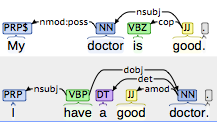
\includegraphics[width=0.40\textwidth]{../images/dep_problem.png}
\caption{Dependency relationships}
\label{fig:dep_rel}
\end{figure}

Label definitions also switch between syntactic and semantic criteria, usually to ensure that central labels such as \texttt{nsubj} have salient lexical dependents, and for the purpose of congruence with analyses of other languages \cite{marneffe_ud_2014}. One important example is the \texttt{root} node, which generally marks the main verb, unless the main verb is copula, in which case \texttt{root} is shifted to the head of the grammatical Complement. A second example is that \texttt{nsubj} is shifted to the grammatical Complement in existential clauses, to avoid marking the experientially empty \emph{there} \cite{halliday_introduction_2004} as the most prominent participant in the clause. Potential issues arising from these decisions can be seen in Figure \ref{fig:dep_rel}. In the first example, \emph{doctor} is problematically analysed as the dependent subject of \emph{good}; in the second example, \emph{good} becomes dependent on \emph{doctor}; in the third example, \emph{doctor} is analysed as \texttt{nsubj} despite not being a grammatical Subject \cite{marneffe_ud_2014}. Moreover, the criteria are variously syntactic and semantic in and of themselves. The \texttt{nsubj} definition is syntactic, while the \texttt{dobj} definition is semantic \cite[see][]{nivre_towards_2015}:

\begin{quotation}\small \singlespacing
\textbf{\texttt{nsubj}}: \emph{A nominal subject is a nominal phrase which is the syntactic subject of a clause.}

\textbf{\texttt{dobj}}: \emph{The direct object of a verb is the noun phrase that denotes the entity acted upon.}
\end{quotation}
%
These inconsistencies are designed to make it possible to quickly extract salient tokens from texts, and to skip words with little experiential meaning in isolation, such as \emph{is} and \emph{there}. For more nuanced functional\hyp{}semantic work, however, such inconsistencies become stumbling blocks that need to be accounted for during corpus querying with verbose sets of conditional rules. While the ergative model of syntax as outlined by \textcite{halliday_introduction_2004} provides a potentially useful means of measuring the extent to which participants are construed as Agents in key processes, the grammar was difficult to operationalise here due to ambiguities in the constituency and dependency grammars. Moreover, the case study demonstrates that critical experiential meanings are made though apparently mundane lemmata such as \emph{be} and \emph{have}. The analysis of the ways in which attributions and ascriptions of \gls{bipolar} vary longitudinally, for example underscores the importance of common words and delicate grammatical distinctions in both the construal of experience and the production and reproduction of a normative community ideology. This issue demonstrates the need for dedicated parsing at the stratum of \glspl{discourse-semantic}---a future possibility described briefly in Chapter \ref{chap:conclusion}.

%If \emph{be} is a key process, or \emph{I} is a key participant, the reason should be investigated. Simply removing these tokens via stopwords list would obscure subtle distinctions in meaning that differentiate \glslink{member}{users} at early and late stages of membership.

%\subsection{Topic modelling}

%Topic modelling is not wholly unproblematic. Topic 13, for example, contained the usernames and nicknames of some veteran members, likely because veterans signed off their posts by writing their name. Jargon terms were also frequent in this topic, as veteran \glspl{member} are more aware of jargon terms than newcomers. Though the increasingly jargonised register of community \glspl{member} is interesting in its own right, this was not the intended job of the topic modeller: \emph{medication} and \emph{meds} are very much the same thing. Similarly, Topics 0 and 21 seemed to contain words relating to social support. Social support, however, is not a major \emph{subtopic} per se, but rather, a common function of veterans' posts. Again, though this provides an insight into longitudinal changes in member roles, it may not necessarily be the kind of insight we were hoping to gain. So long as researchers remain aware of these limitations, however, topic modelling remains a novel way to categorise corpus texts, and to understand corpus composition. Creating sub\glspl{corpus} based on topic modeller output seems an especially promising strategy: with news \glspl{corpus}, for example, this kind of approach could be used to compare the language used in sports reporting, politics reporting, finance reporting, and so forth. CADS could even use topic modelling as a means of splitting and balancing very large general \glspl{corpus}.

\subsubsection{Limitations in available systemic\hyp{}functional resources}

For the \sctext{Transitivity} analysis in Chapter \ref{chap:experiential}, Events were identified by searching for words in grammatical positions that correspond with Events in the \gls{SFG}. Simple wordlists were then used to group the Events into Process Types. Such an approach does not account for the fact that the same verb can realise multiple process types (\emph{I feel sick}\slash\emph{I feel leather}---recall Section \ref{sect:sfl}). Distinguishing between Process Types is a notoriously difficult task, with poor inter\hyp{}rater reliability even for trained human annotators \cite{gwilliams_indeterminacy_2015,odonnell_survey_2009}. Adding to the difficulty of this task is that two competing descriptions of Process Type exist within \gls{SFL}, generally known as the Cardiff and Sydney Grammars respectively \cite{costetchi_method_2013}. Wordlists were drawn from the Process Type Database \cite{neale_more_2002}, which uses the Cardiff Grammar, while the theoretical framework used was the Hallidayan Sydney Grammar \cite[as described in e.g.][]{eggins_introduction_2004,halliday_introduction_2004}. As such, behavioural processes were not identified or differentiated from the Process Types that subsume them in the Cardiff Grammar. More complete computational resources for Process Type identification as per the Sydney Grammar, such as recent work outlined by \textcite{matthiessen_extending_2014}, remain to be put under version control, and packaged and distributed in a useful computational form.

\subsubsection{The limits of lexicogrammatical querying}

A key limitation of the developed methodology in general is that searching lexicogrammatical information with the aim of learning about \glspl{discourse-semantic} can ultimately only provide a partial account of meaning\hyp{}making. This account is also biased toward text with a greater degree of congruence between wording and meaning: an interaction rich in politeness marking, or a highly nominalised piece of science writing, pose additional challenges for researchers interested in semantic phenomena. For the analysis of the \glslink{Forum}{Bipolar Forum}, the major strategy used to quantify semantic information was to query progressively more delicate components of the \gls{lexicogrammar}. At a number of points during the case study, however, it was not possible to further extend the delicacy of queries in order to disambiguate the meaning or function of a clause. The best example of this issue is in the analysis of \emph{I $+$ would $+$ Adjunct} declaratives (see Section \ref{sect:modalisation}). Here, the same lexicogrammatical feature set can index very different meanings and functions, based on co\hyp{}text, context and the experiential likelihood of the construal. Automated lexicogrammatical querying, therefore, cannot easily distinguish between the longitudinal changes in the typical function of the construction. This is a known property of modalised declaratives and proposals more generally: in order to make a command discretionary for the addressee, the speaker must shift to the indicative Mood to allow modalisation. Doing so creates ambiguity between proposal and proposition \cite{halliday_introduction_2004}: \emph{I would occassionally go to sleep for as much as 24 hours} describes past behaviour, but in another context, could grammatically function as advice. It must then be disambiguated, either through human interpretation of the semantics of the clause (\emph{Is this plausible as advice?}), or by considering the neighbouring moves within the interaction (it would, for example, be very unusual to dispense advice in the middle of a recounting of a past event).

Using existing tools to automatically resolve this kind of ambiguity is difficult. The query could be extended in delicacy and complexity to capture co\hyp{}occurring features such as a second person pronoun in the Complement, which would increase the likelihood that the intended function is advice (\emph{I would go back to your doc}). This approach is unlikely to be accurate, scalable, or reusable, however. Other approaches, such as supervised automatic classification, involve manually labelling a sample of instances to use as training data. This is more scalable, but can be a resource\hyp{}intensive and computationally complex undertaking. For now, this kind of ambiguity in English \gls{lexicogrammar} demonstrates the continuing necessity of manual classification of corpus instances. Looking forward, however, it seems that the most logical way to address the issue is to build tools that annotate the semantic stratum directly. This possibility is briefly described in Chapter \ref{chap:conclusion}.

Because semantic information could not be directly accessed through the developed methodology, the linguistic sites of change identified over the course of the case study only form a small fraction of the total set of \gls{discourse-semantic} meanings at risk over the membership course. The extent to which the findings capture the total meaning potential of the community is also constrained by limitations of scope: only a handful of linguistic phenomena, chosen mostly from very frequent features in the \gls{lexicogrammar}, were analysed in detail. Other parts of the meaning\hyp{}making process may have therefore escaped attention for any number of reasons. First, some less common meanings at risk may have been buried within very large lists of results. Second, some patterns in meaning are realised through combinations of lexicogrammatical features that were not searched during the case study: though it is possible to calculate keyness for entire nominal groups, or for key Thing\slash Event pairs, these strategies were not pursued. It also needs to be kept in mind that some aspects of meaning were filtered out of the texts before analysis had begun, during the \gls{corpus} creation process. Two examples are emoticons and hyperlinks, both of which are capable of doing important pragmatic work \cite{koteyko2015performing,schandorf_mediated_2013}.

% call this 'agnate realisations'
\subsubsection{Rank shift and grammatical metaphor}

Another encountered issue was rank shift---that is, the realisation of a meaning at an incongruent stratum \cite{halliday_introduction_2004}. If a researcher is interested in the ways in which \emph{pdocs} are appraised in the text, for example, he\slash she may begin by finding all adjectival modifiers within a nominal group headed by \emph{pdoc} (as in Example 1, below). Similar kinds of appraisal, however, can also take place at clause level (Example 2), through embedded clauses (Example 3) or at the level of clause complex (Example 4).

\begin{multicols}{2}
\begin{enumerate}
\footnotesize
\setlength\itemsep{-0.5em}
\item My really lovely pdoc helped me out. %group level appraisal
\item My pdoc is really lovely and helped me out. %clause level
\item My pdoc, being really lovely, helped me out. %embedded clause
\item My pdoc helped me out. She's really lovely. %clause complex
\end{enumerate}
\end{multicols}
%
\noindent In each case, more complex kinds of interrogation are required in order to map \emph{really lovely} to \emph{my pdoc}. Moreover, even the most nuanced querying cannot lead to certainty in statements regarding the ways meanings are typically made, as potential realisations of the Appraisal, and thus, potential lexicogrammatical queries, are limitless. As a result, in this investigation, and most \gls{CADS} more generally, the discourse being analysed is for the most part only that which is realised congruently. Given the high frequency of incongruent realisation in general, this is indeed a serious concern. Furthermore, according to \gls{SFL}, meanings made through rank shift or incongruence are deliberate speaker choices, with significant interpersonal, experiential and textual motivations. If they are systematically not located by interrogation queries, certain kinds of meanings may go consistently unseen. This limitation becomes more serious again when we consider the role\hyp{}relationships under investigation in the \glslink{Forum}{Bipolar Forum}. Unequal role relationships result in the need for newer \glspl{member} to \emph{disperse} the mood system when issuing commands: demands for information are dressed as offerings of information:

\begin{quote}
\emph{I would appreciate any advice~~~~~~~~~~~~~~~~~~~~~~I wonder if this is normal!?}
\end{quote}

This point is also made by \textcite{slade_emergency_2008}, in the context of the ways in which healthcare consumers may relate symptoms and illnesses to themselves:

\begin{quote} \small \singlespacing
When a person describes a disease or its symptoms, they can describe it in a number of ways; as part of the goings\hyp{}on in their external world (i.e. material or behavioural process) as part of the goings\hyp{}on in the person's internal world (i.e. mental process), as something that they own (i.e. relational possessive process) or as a characteristic or something that can be related to some other thing (i.e. relational process) \parencite*[p.~290]{slade_emergency_2008}.
\end{quote}
%
The case study charted attribution of \emph{bipolar} via relational processes, with the afflicted occupying one participant role and the disorder occupying another. Other kinds of ascriptions (e.g. \emph{my bipolar}, \emph{this condition that I have}), were ignored. While nothing stops the researcher from searching for multiple kinds of realisations of a given meaning, iterative developing and checking of query accuracy can be a time consuming process. At the same time, it can lead to unmanageably large sets of disparate results. Moreover, these results cannot be compressed without oversimplifying how language works. When investigating the \emph{diagnose} process (Section \ref{sect:diag}), it was found that the most common modifiers are temporal. The nominalised form, \emph{diagnosis}, however, more commonly selects modifiers of veracity. How, then, can we combine these two results, and quantify all modification of the semantic unit of diagnosis (which may be either process or participant)? One solution would be to turn adverbial modifiers into their adjectival variant (\emph{accurately $\rightarrow$ accurate}), and then to merge the results. This quickly runs aground, however: because \emph{diagnose} is more often realised (congruently) as a process, the frequencies may now be biased toward the congruent. To add another complication, the circumstances selected by the \emph{diagnose} process are not static, but vary by membership stage. Therefore, while it is possible to say that diagnosis is increasingly framed with respect to its veracity (because veteran \glspl{member} modify the process that way, and because they increasingly use the participant form, which co\hyp{}occurs with veracity modifiers generally), it is not yet possible to describe the semantic unit of diagnosis accurately within a single, two\hyp{}dimensional representation.

A final, related issue is that grammatical categories operationalised as search criteria, even within a functional grammar, do not necessarily correspond with their sociological significance. \textcite{van_leeuwen_representation_1996} reminds us, for instance, that there is a difference between the sociological and grammatical conceptualisations of agency. First, not all agentive constructions imply agency in the sociological sense. Concordancing of first person Agents in first \glspl{post} shows many examples of the disparity (\emph{I can never make decisions and i worry all the time about everything}; \emph{I just wish i could feel one way and not so many different ones if that makes any sense}; \emph{once they gave me a small electric shock i screamed and i couldn't go on with the test}). Second, agency in the sociological sense is not exclusively construed through grammatical agency: possessives and preposition phrases, for example, can accomplish in the agency sociological sense (\emph{my decision was to discontinue lithium}). 

%Decisions to structure the corpus in one way obscure the influence of other variables: all first posts were grouped together here, though some people had been non-posting \glspl{member} for months before posting. Some first posts initiated new threads, and others were replies to other threads. That said, so long as all possible metadata is collected and stored within texts,

\subsubsection{The influence of genre}

When comparing the results of Chapter \ref{chap:introdata} with those of Chapters \ref{chap:interpersonal} and \ref{chap:experiential}, it is clear that genre, while playing a central role in setting the probabilities for lexicogrammatical and \gls{discourse-semantic} features of genre stages, is not well\hyp{}captured by the developed corpus linguistic methods. When new \glslink{member}{users} initiate a `first \gls{post} \gls{thread}', for example, the organisation and content of the \gls{post} may conform to a generic structure related to what has been found in investigations of other \glspl{OSG}. As in \textcite{varga2014grieving}, \glspl{post} frequently provide a narrative medical history. Encounters with formal healthcare institutions, and the diagnosis event, are then presented, in line with previous studies of bipolar \glspl{forum} \cite[e.g.][]{vayreda_social_2009}. As found by \textcite{horne_doing_2009}, users may then go on to describe a current problem. In the \glslink{Forum}{Bipolar Forum}, these problems are diverse, including symptoms, side\hyp{}effects, relationship issues, work issues, or problems with health professionals and\slash or institutions. Finally, users commonly make a demand for information or support on other members. Given the low social status of newcomers, these requests are realised by any of a range of agnate linguistic structures: they may be overt or relatively implicit, with statements hinting at a need for further information or social support often standing in for more direct requests for advice. An element of recursivity in the generic structure allows users to contextualise and formulate multiple problems that require responses from others.

The influence of genre on lexicogrammar can be seen at a number of points throughout Chapters \ref{chap:introdata}--\ref{chap:experiential}. In terms of shallow features, the first few \glspl{post} to the \gls{Forum} were found to be in many respects more formal (longer words; higher proportion of nouns; higher lexical density) than those that follow. Lexically, \emph{diagnose} as a process is very key in first \glspl{post}, appearing within the \sctext{Orientation} stage, as many new \glspl{member} frame their entry in terms of a recent or possible diagnosis. \emph{Anyone} features as a prominent participant in the \sctext{Request} stage as a means of soliciting contributions from others (\emph{Can anyone explain this to me?}); \emph{thank} and \emph{appreciate} become key processes in second and third posts as users follow up to the responses generated by their first. Though the metadata embedded in the parsed corpus contains information regarding the thread, and the position of the \gls{post} within it, how to use this data to either investigate or control for generic influence remains unknown.

% todo: delete?
\subsubsection{Multimodality}

Though the original \gls{HTML} is preserved, making it possible to view any search result in something very similar to its original context, \gls{corpus} interrogation typically involves counting so many strings of text that contextualised reading of each is unfeasible. When analysing plain text without accompanying metadata, a researcher may miss key semiotic features that shape the way meanings are made. Throughout the case study, though some member quotes were presented multimodally where possible, no systematic analysis of the influence of these features was performed. Given that join date, post\hyp{}count, and a visualisation of post\hyp{}count as a green `progress bar', are the most obvious ways in which membership stage is communicated, it is certainly a limitation that the thesis did not provide an account of how these features may work to reinforce and\slash or negotiate speaker roles and identities.

It should also be noted that the well\hyp{}known criticism of \gls{CL} methods as obscuring (multimodal) context are not inherent to the approach, but are in fact the result of limitations in software design. \texttt{corpkit}, for example, can show arbitrary metadata features for a sentence alongside its representation within a concordance. Recent work in multimodal \gls{SFL} \cite[e.g.][]{hiippala2015,hiippala2016,ohalloran_multimodal_2013} has demonstrated the possibility of extending such methods to allow display of the original, multimodal texts themselves. In this approach, \gls{XML} documents store page layout, audiovisual information and text in such a way that the content remains searchable using \gls{CL} methods. Looking forward, it would be feasible to link parsed versions of texts to their copies within the multimodal \gls{corpus}, so that researchers could switch between monomodal and multimodal views of \gls{corpus} interrogations. Searches could also be restricted to texts co\hyp{}occurring with a given multimodal feature, as \texttt{corpkit} allows with other metadata features. 

%Despite this possibility, analysis of the ways in which multimodal content makes meaning is still a largely manual task.

\subsubsection{SFL, the individual and the mind}

The final part of the research design requiring critical reflection is the use of \gls{SFL} as a theory that models ontogenetic language change. As explained in Section \ref{sect:sfl}, \gls{SFL} encompasses both a grammar (in the form of the \gls{SFG}) and conceptualisation of the relationship between language, text, language users, and context. In many repsects, the grammar provided by \gls{SFL}---the \gls{SFG}---provides an exemplary framework for dividing language use into metafunctions, and for relating metafunctions to semantics and wordings in a systematic way. It is particularly useful in a \gls{CL} context, where the investigation must proceed in some logical order (here, along metafunctional lines, and toward delicacy on the instantiative cline), and where searching must be lexicogrammatical, even when a primary interest is \glspl{discourse-semantic}. As a theory of language, however, \gls{SFL},\endnote{I am referring to Hallidayan SFL here---Fawcett, within the Cardiff tradition, has attempted to provide a link between SFL and cognition \parencite*[e.g.][]{fawcett1980cognitive}.} is centred on modelling \emph{language as social action} \cite{halliday1978language}: it explains how language accomplishes meaning, in the form of the negotiation of relationships (Tenor), the construal of experience (Field) and reflexive self organisation (Mode).

At issue, first, is that the Tenor dimension of register does not model the identity of individual speakers within an interaction. Rather, the Tenor of discourse is the \emph{sets of role\hyp{}relationships}, as interpreted from social semiotics \cite{halliday_language_1989}. In systemic terminology, it is therefore not accurate to say that a \gls{Forum} \glslink{member}{user}'s register shifts over the membership course. Instead, a language user, while gradually shifting from newcomer to veteran status, simply enters into interactions within the \gls{Forum}, and during each, makes linguistic choices that reflect his\slash her relative position within the social hierarchies of the interaction and the broader context of the \glslink{Forum}{board}.

Because \gls{SFL} does little modelling of the individual, it also makes little effort to engage with the cognitive processes that bring about speech (exceptions here work by \textcite{crocker2016information,degaetano-ortlieb_data_2014}. In fact, \textcite{matthiessen1998construing} advances an argument that \emph{the mind} is, for the most part, a linguistic construct grounded not in cognitive science, but simply in lay perception of the world:

\begin{quote}\singlespacing\small
But `what is the mind'---or more explicitly, what kind of experience is construed as `the mind', and how is it located relative to related categories of experience? The most general answer is that `the mind' is a linguistic construct---a category of our experience that we construe for ourself by means of our everyday \gls{lexicogrammar} \parencite*[p.~327]{matthiessen1998construing}.
\end{quote}
%
Ultimately, therefore, \gls{SFL} can be characterised as an historical\hyp{}material interpretation of semiotic systems, with the individual and his\slash her mind understood as little more than the set of Tenor roles he\slash she has filled within the \gls{corpus}.

This theoretical orientation toward the material and the semiotic \cite{thompson2001interview} places hard limits on what can be said about individuals' language use within the \glslink{Forum}{community}. The first constraint is on what can be contained within an account of the consumer journey. In \gls{SFL}, the only parts of the \gls{consumer} journey that are available for analysis are those where the \gls{consumer} engages in an act of entextualisation---a recorded encounter within some social space. The inner or unrecorded paths within the journey---that portion comprised of a consumer's unexpressed expectations, fears and beliefs---is inaccessible. The second constraint is on connecting language use to thought, and therefore, to key notions in \gls{HC} research such as psycho\hyp{}education or health literacy. While other theories conceptualise \gls{OSG} use as a kind of talk therapy \cite{kaufman2016producing}, and while \gls{SFL} can be fruitfully used to locate and explain the socio\hyp{}semiotic processes of therapeutic talk, there is little room within the theory to argue that language change patterns with cognitive change, and therefore, that the observed patterns may in and of themselves be examples of positive or negative health outcomes. Accordingly, in future research intending to relate speakers' linguistic practices to the attainment of health outcomes, it may be useful to better distinguish between the \gls{SFG} and \gls{SFL}. More specifically, a researcher could adopt the grammar as a means of distinguishing between kinds of meaning and their realisation in the words and wordings of texts, but undertake the task of connecting language use to cognition through an alternative (psycholinguistic) lens.

\section{Summary}

In this and the previous chapters, I discussed an investigation of the \glslink{forum}{Bipolar Forum} as a linguistic \gls{corpus}. Change over the course of membership was found to be both interpersonal and experiential. \glslink{member}{Users} constantly renegotiate their status within the \glslink{forum}{community} through \sctext{Mood} and \sctext{Modality} choices. Experientially, \glslink{member}{users} demonstrate shifts in the kinds of participants and processes most commonly construed, but also the way these participants and processes are discursively framed. A reflection on the theory and methodology of the study highlighted key methodological challenges in extracting meaningful information from annotated \glspl{corpus}, and key theoretical challenges in the use of \gls{SFL} as a theory of ontogenetic linguistic change.

In the next chapter, I outline the implications of the thesis and its associated tools and methods for \gls{CL}, \gls{SFL} and \gls{HC} research.

%Generally, findings echo claims made in recent \gls{OSG} literature. The novel methodological components of the investigation reveal how it is possible to find reproducible, quantifiable support for claims that were originally based on qualitative interpretation of small samples of \glspl{OSG}. A short analysis of generic features of first contributions and the replies they receive has demonstrated that ...
